\documentclass{beamer}
\usetheme{Boadilla}

\usepackage{hyperref}
\hypersetup{
  colorlinks = true,
  urlcolor   = blue,
  linkcolor  = blue,
  citecolor  = red
}

% --------------------------------------------------------

\title{Modern data analytics}
\subtitle{COVID-19 analysis}
\author{Sebastiaan Van den Broeck}
\institute{KUL}
\date{\today}

% --------------------------------------------------------

\begin{document}

% Title slide
\begin{frame}
\titlepage
\end{frame}

% Table of content
\begin{frame}
\frametitle{Outline}
\tableofcontents
\end{frame}

% Introduction
\section{Introduction}
\begin{frame}
\frametitle{Introduction}
This is the introduction
\end{frame}

% Methodology
\section{Methodology}
\begin{frame}
\frametitle{Methodology}

\begin{figure}
\centering
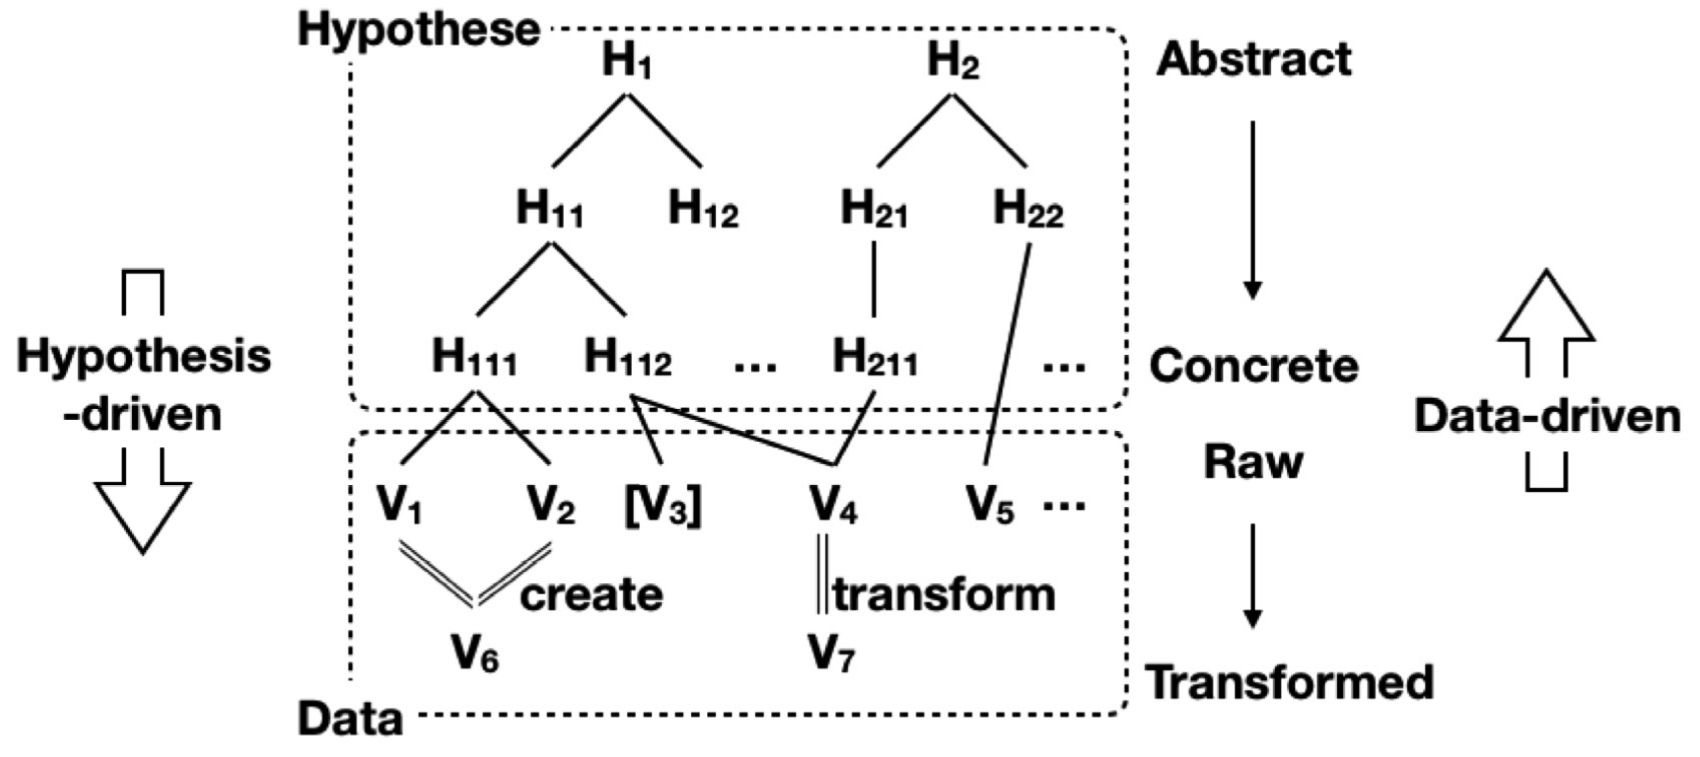
\includegraphics[width=0.8\linewidth]{../visualizations/hypothesis_space_data_space.png}
\end{figure}

\end{frame}

% Data sources
\section{Data sources}
\begin{frame}
\frametitle{Data sources}

\begin{enumerate}
\item \href{https://github.com/nytimes/covid-19-data}{The COVID-19 dataset}
\item \href{https://apps.bea.gov/regional/downloadzip.cfm}{Economical information}
\item \href{https://zenodo.org/record/6411336\#.YvUG14VBzCl}{The COVID-19 OpenSky dataset}
\item \href{https://github.com/allenai/cord19}{The CORD-19 dataset}
\end{enumerate}

\end{frame}

% Exploratory data analysis
\section{Exploratory data analysis}
\begin{frame}
\frametitle{Exploratory data analysis}

\end{frame}

% Graph mining
\section{Graph mining}
\begin{frame}
\frametitle{Graph mining}

\begin{figure}
\centering
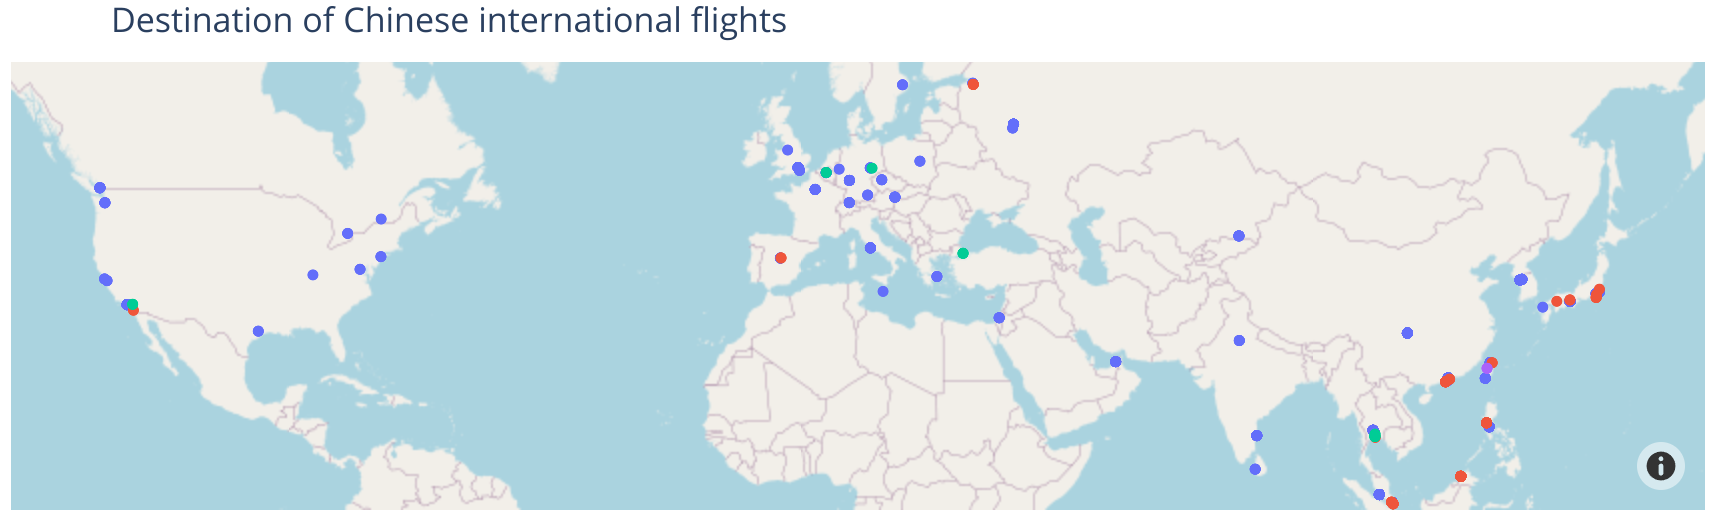
\includegraphics[width=0.8\linewidth]{../visualizations/chinese_flights_screenshot.png}
\end{figure}

\end{frame}


\begin{frame}
\frametitle{Graph mining}

\begin{itemize}
  \item Degree \hspace{36px} $c_D (i) = \sum_j^N x_{ij}$ \\
    \hspace{72px} where $i, j$ are nodes and $x$ is the adjacency matrix.
  \vfill
  \item Betweenness \hspace{10px} $c_B (i) = \sum_{s, t \in i} \dfrac{\sigma (s, t | i)}{\sigma (s, t)}$ \\
    \hspace{72px} where $i$ is a node, $s$ and $t$ are source and target \\
    \hspace{72px} nodes, $\sigma (s, t)$ is the number of shortest paths \\
    \hspace{72px} between the source and target and $\sigma (s, t | v)$ is the \\
    \hspace{72px} number of shortest paths passing through the node $v$.
  \vfill
  \item Closeness \hspace{25px} $c_C(i) = \left[ \sum_j^N d(i, j) \right]^{-1}$ \\
    \hspace{72px} where $d$ is a distance metric.
\end{itemize}

\vfill

(Brandes, 2008; Opsahl et al., 2010)

\end{frame}


\begin{frame}
\frametitle{Graph mining - the code}

\begin{figure}
\centering
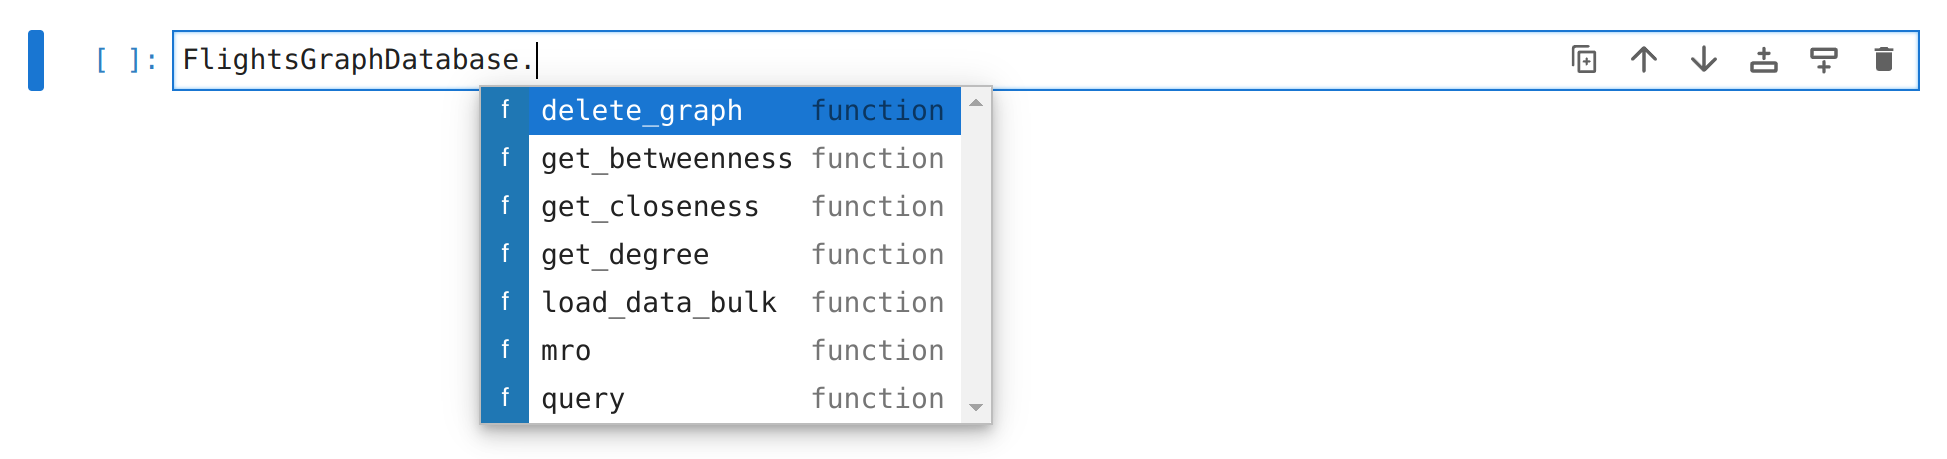
\includegraphics[width=0.8\linewidth]{../visualizations/graph_class_methods.png}
\vfill
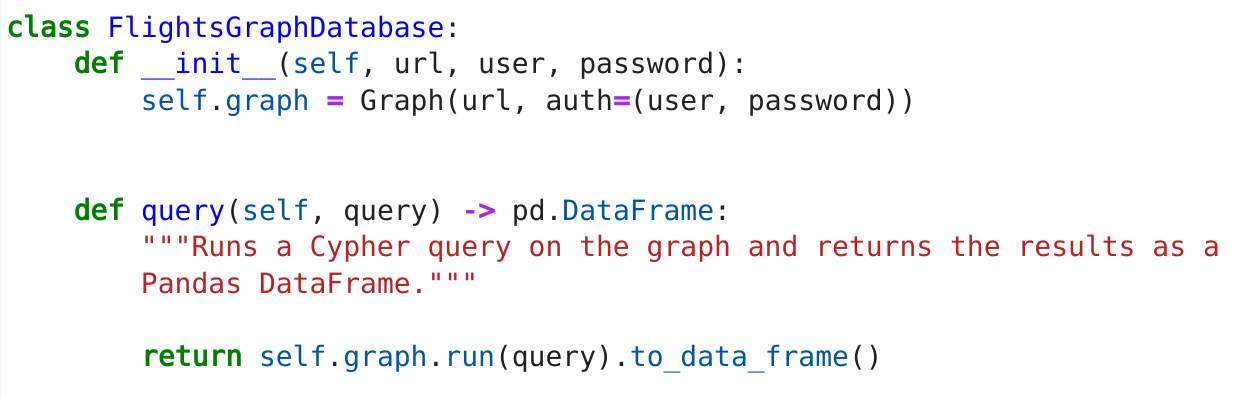
\includegraphics[width=0.8\linewidth]{../visualizations/graph_class_code.png}
\end{figure}

\end{frame}


\begin{frame}
\frametitle{Graph mining - degree centrality}

\begin{figure}
\centering
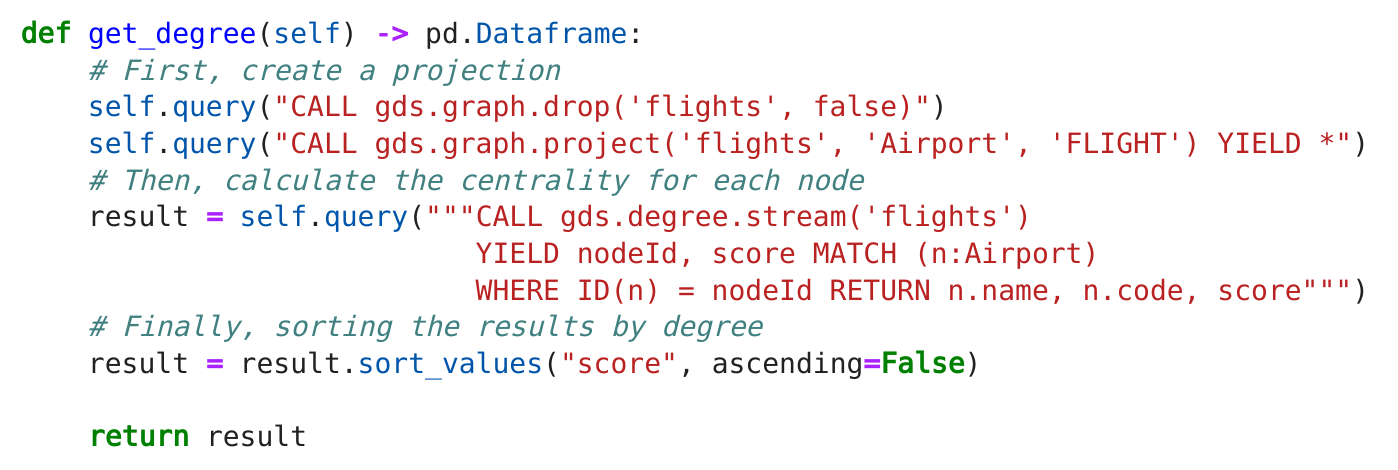
\includegraphics[width=0.6\linewidth]{../visualizations/get_degree_code.png}
\vfill
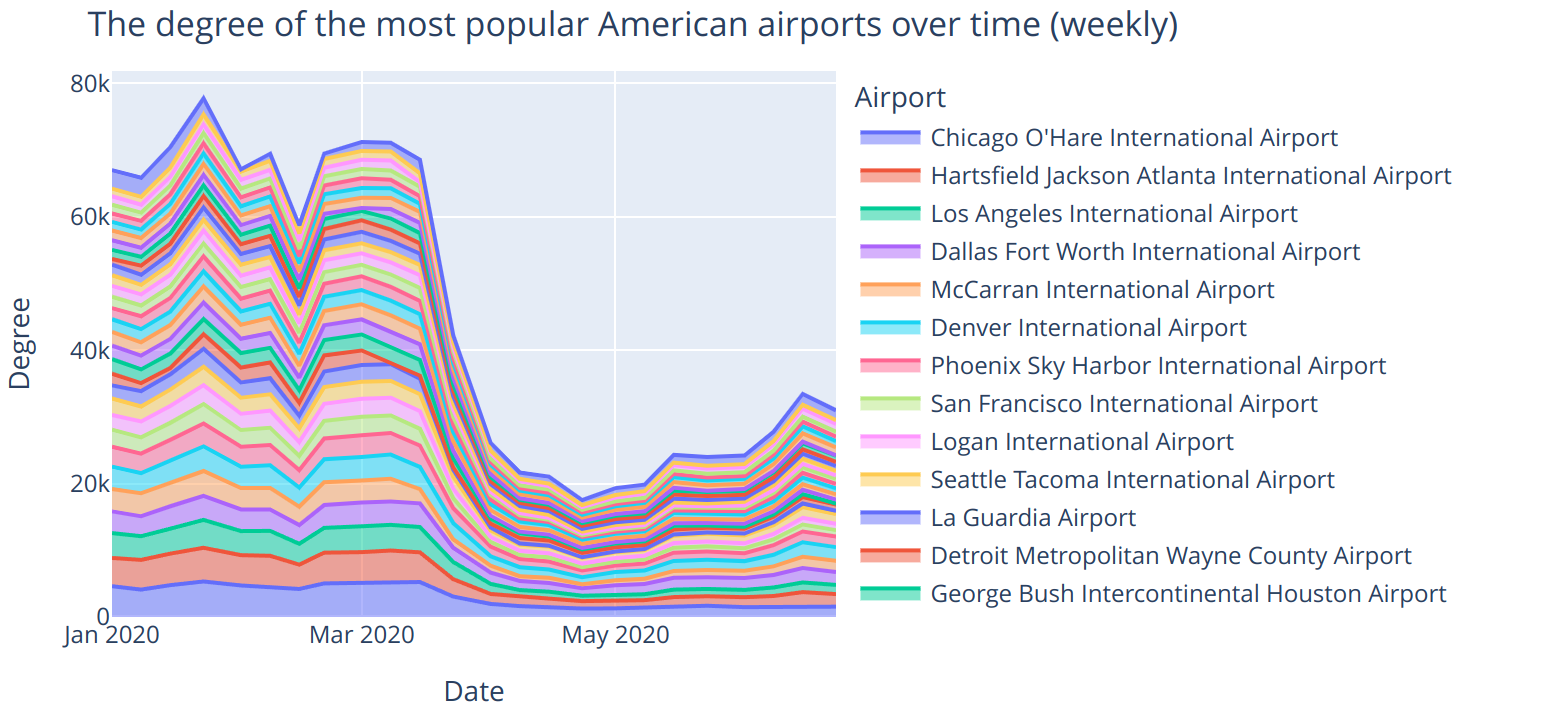
\includegraphics[width=0.6\linewidth]{../visualizations/degree_screenshot.png}
\end{figure}

\end{frame}


\begin{frame}
\frametitle{Graph mining - betweenness centrality}

\begin{figure}
\centering
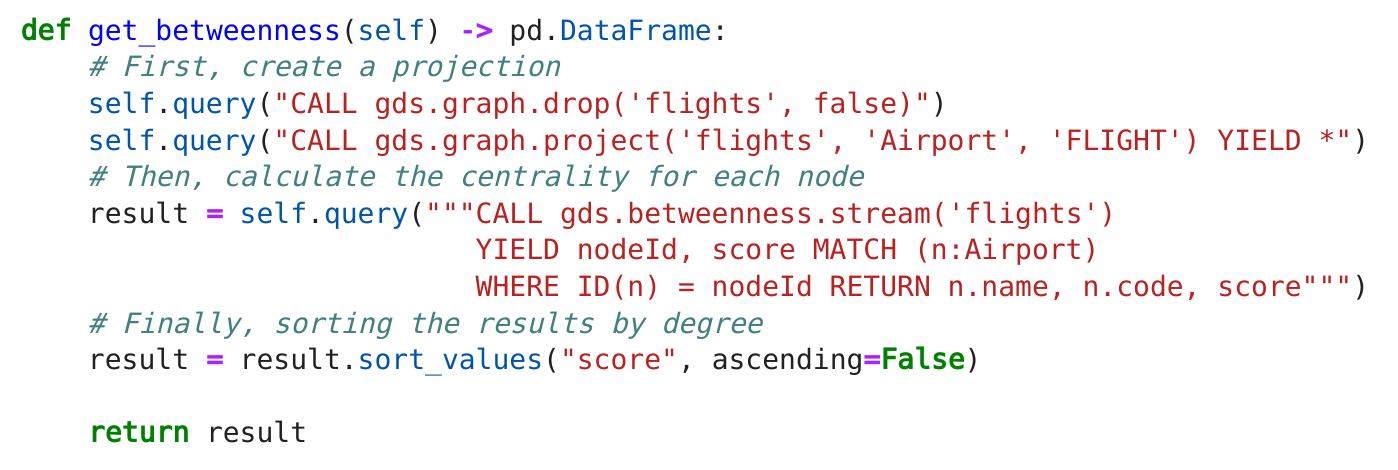
\includegraphics[width=0.6\linewidth]{../visualizations/get_betweenness_code.png}
\vfill
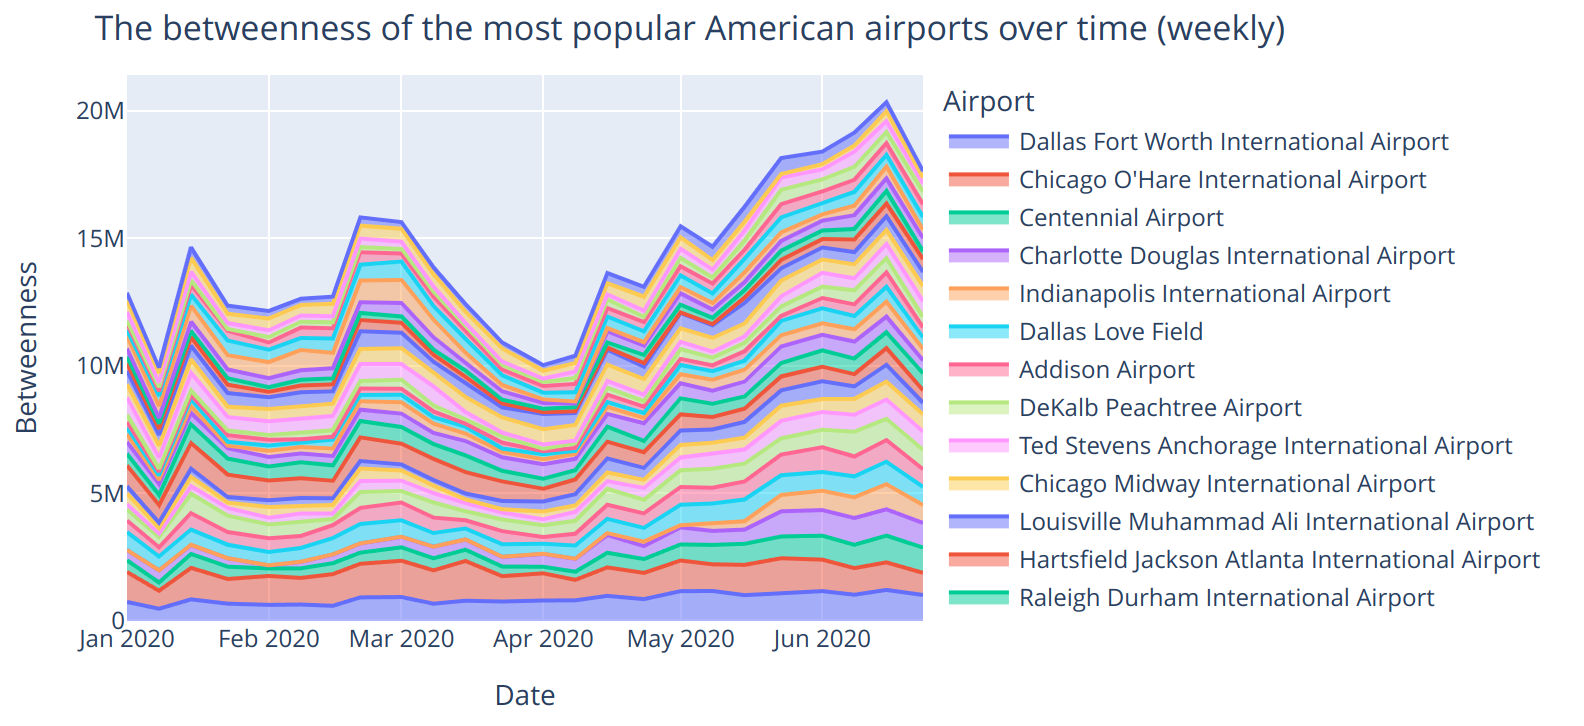
\includegraphics[width=0.6\linewidth]{../visualizations/betweenness_screenshot.png}
\end{figure}

\end{frame}


\begin{frame}
\frametitle{Graph mining - closeness centrality}

\begin{figure}
\centering
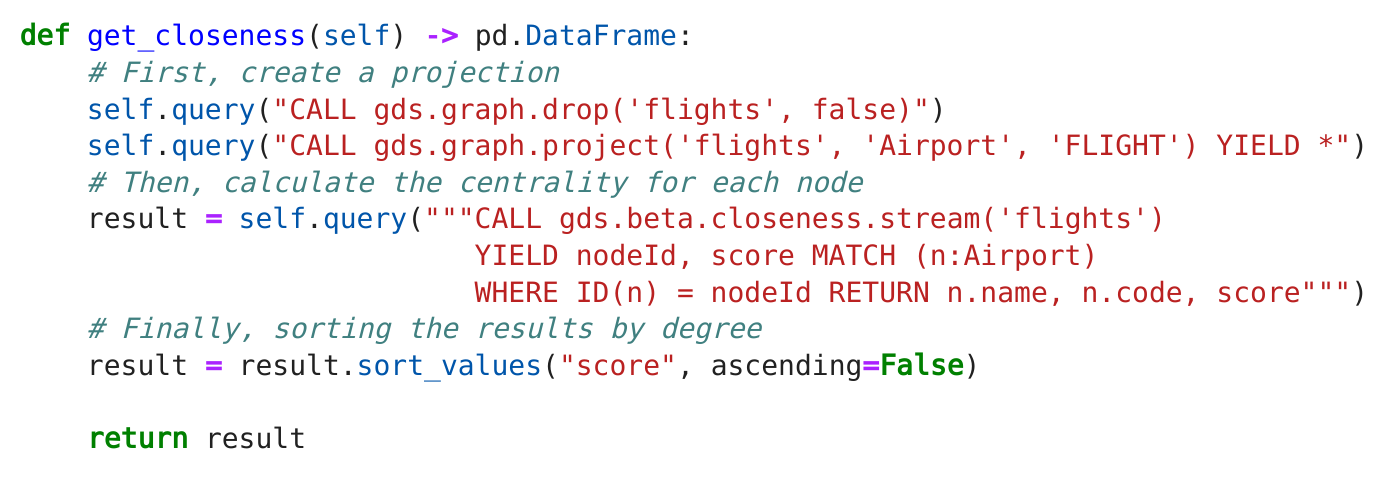
\includegraphics[width=0.6\linewidth]{../visualizations/get_closeness_code.png}
\vfill
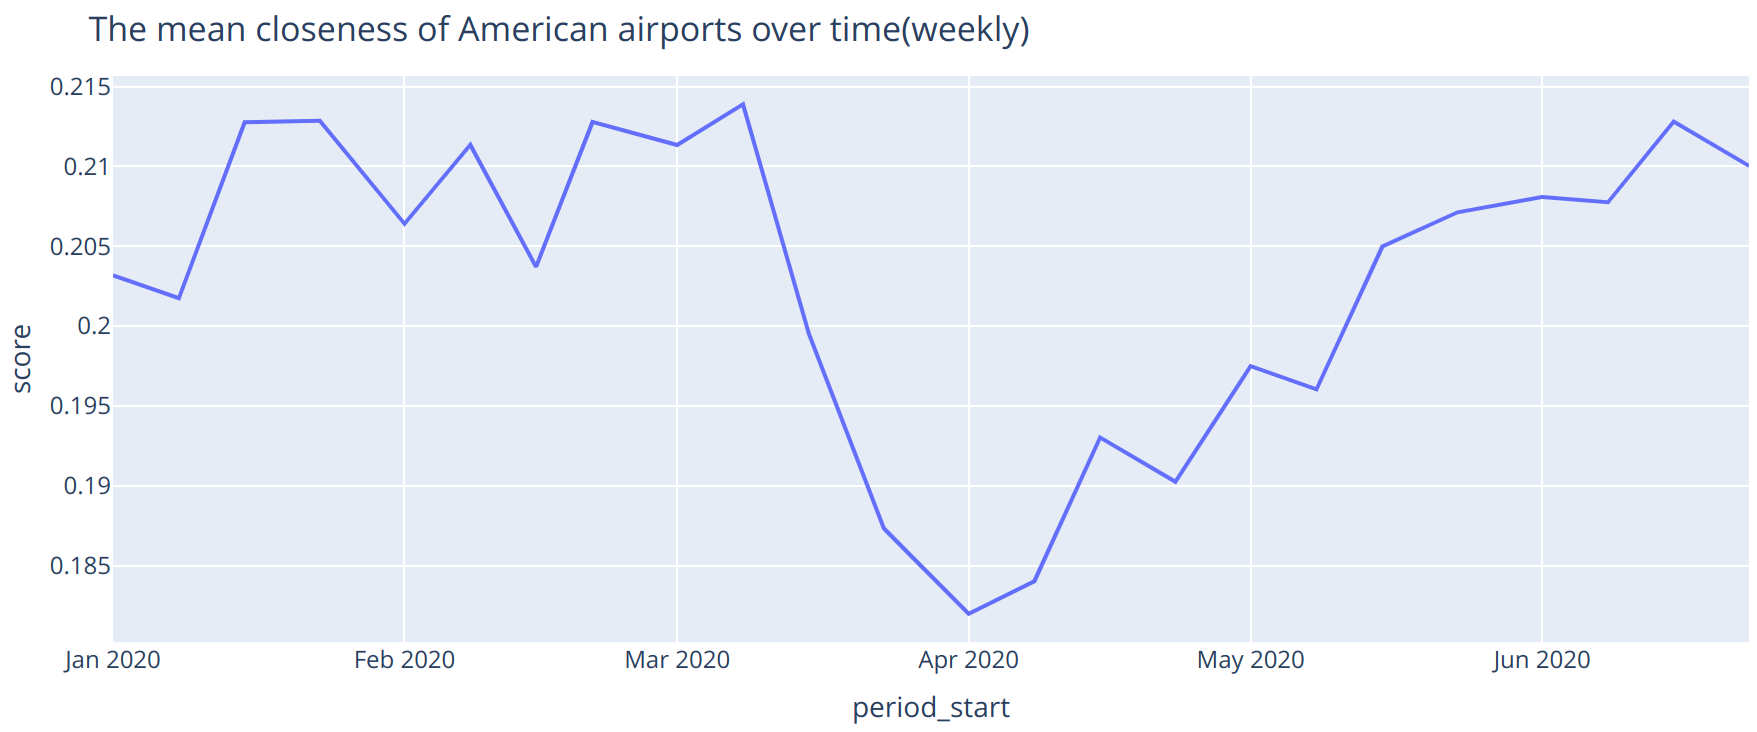
\includegraphics[width=0.6\linewidth]{../visualizations/closeness_screenshot.png}
\end{figure}

\end{frame}

% Text mining
\section{Text mining}
\begin{frame}
\frametitle{Text mining - preprocessing}

\begin{figure}
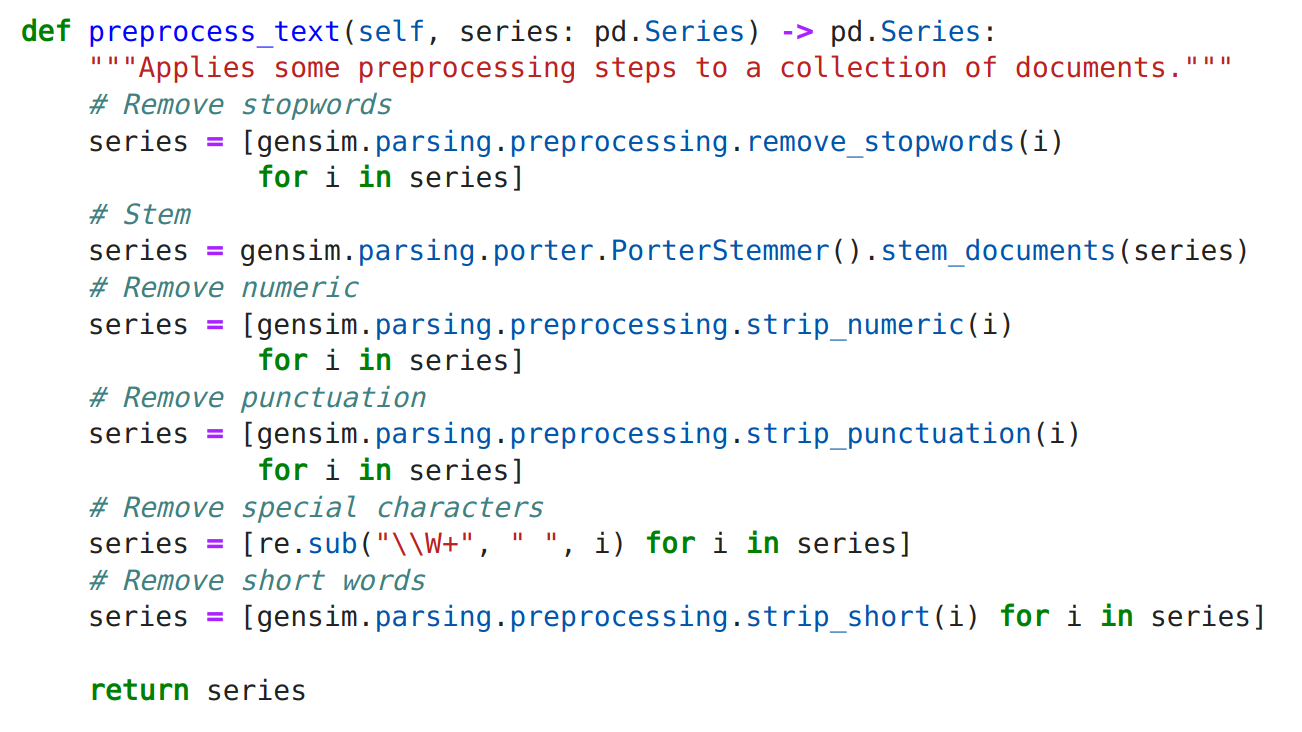
\includegraphics[width=0.6\linewidth]{../visualizations/preprocess_text_code.png}
\end{figure}

\end{frame}


\begin{frame}

\frametitle{Text mining - latent dirichet allocation}
This is a frame.

\end{frame}

% Conclusion
\section{Conclusion}
\begin{frame}
\frametitle{Conclusion}
This is a frame.
\end{frame}

% Sources
\begin{frame}
\frametitle{Sources}
\end{frame}

\end{document}

